\documentclass{article}
% We will use NIPS submission format
\usepackage{nips13submit_e,times}
% for hyperlinks
\usepackage{hyperref}
\usepackage{url}
% For figures
\usepackage{graphicx}
\usepackage{subfigure}
% math packages
\usepackage{amsmath}
\usepackage{amsfonts}
\usepackage{amsopn}
\usepackage{ifthen}
\usepackage{natbib}

\title{Machine Learning Project II by Group KATHMANDU}

\author{
  Jade Copet\\
  EPFL \\
  \texttt{jade.copet@epfl.com} \\
  \And
  Merlin Nimier David\\
  EPFL \\
  \texttt{merlin.nimier-david@epfl.com} \\
  \And
  Krishna Raj Sapkota\\
  EPFL \\
  \texttt{krishna.sapkota@epfl.com} \\
}

\nipsfinalcopy

\begin{document}
\maketitle



\begin{abstract}
\end{abstract}



\section{Song recommendation}

  \subsection{Dataset description}
  \textbf{Objective}: The song recommendation dataset represents the musical habits of users on a musical streaming service. We are given a large number of (user, artist, listening count) triplets, as well as a friendship graph encoding the connections between users. Our goal is to use this training data to perform:

  \begin{itemize}
    \item \textit{Weak} generalization: for existing users, predict the listening counts for unobserved (user, artist) pairs.
    \item \textit{Strong} generalization: for unknown users, predict the listening counts. We may use the friendship data.
  \end{itemize}

  \textbf{About the data}: The listening counts matrix $Y$ covers $1774$ users and $15085$ artists. It is very sparse, as we observe only $69617$ triplets (density of $0.2\%$). The friendship graph $G$ is given in the form of a symmetric $1774 \times 1774$ adjacency matrix, where $G_{i, j} = G_{j, i} = 1$ if users $i$ and $j$ are connected.\\

  Artists have listening counts ranging from $1$ to $2274039$, the most listened artist being Britney Spears (for some reason). Over all observations, before any outlier removal, the average count is 707 while the median count is 278.\\

  TODO: explain carefully how we handled unobserved data.

  \textbf{Error measure}: Both weak and strong prediction involve generating, for a given set of (user, artist) pairs, predicted listening counts. We use mean \textbf{RMSE} as our main error measure. Given a predicted triplets $\hat{Y}$, we compute the RMSE of the residuals on nonzero elements of the target sparse matrix $Y$.\\

  \subsection{Dataset analysis and preprocessing}
  Examining the dataset, we noticed that user $385$ had listened to artist $9162$ a whopping $352698$ times. Assuming an average song duration of $3$ minutes, user $385$ have supposedly spent the equivalent of two full years listening to \textit{Depeche Mode}. It was then necessary to remove such outliers before carrying out any learning.

  Several Machine Learning techniques rely on the assumption that data follows a Gaussian distribution. Applying a $\log$ transform to listening counts brought all counts back to a common scale.

  \begin{figure}[ht]
    \center
    \subfigure{
      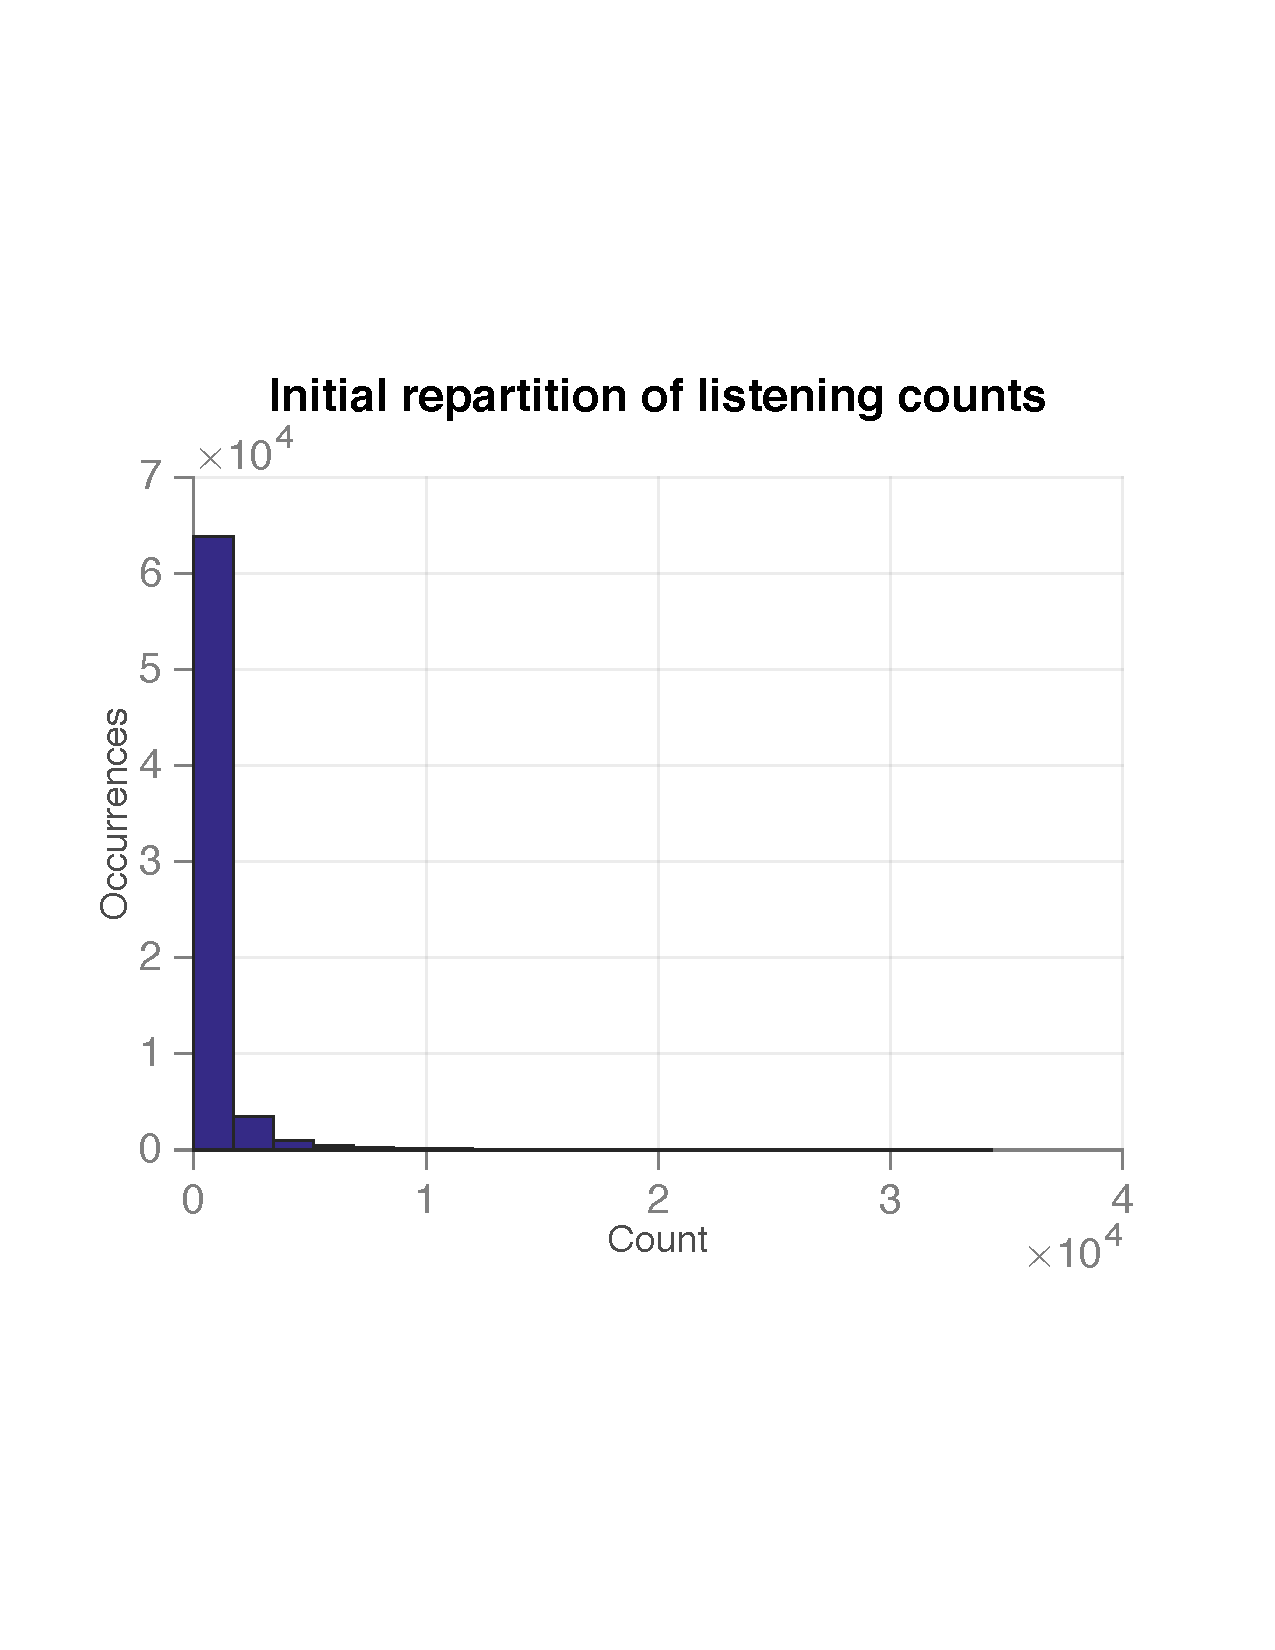
\includegraphics[width=2.5in]{figures/recommendation/unnormalized-counts.pdf}
    }
    \subfigure{
      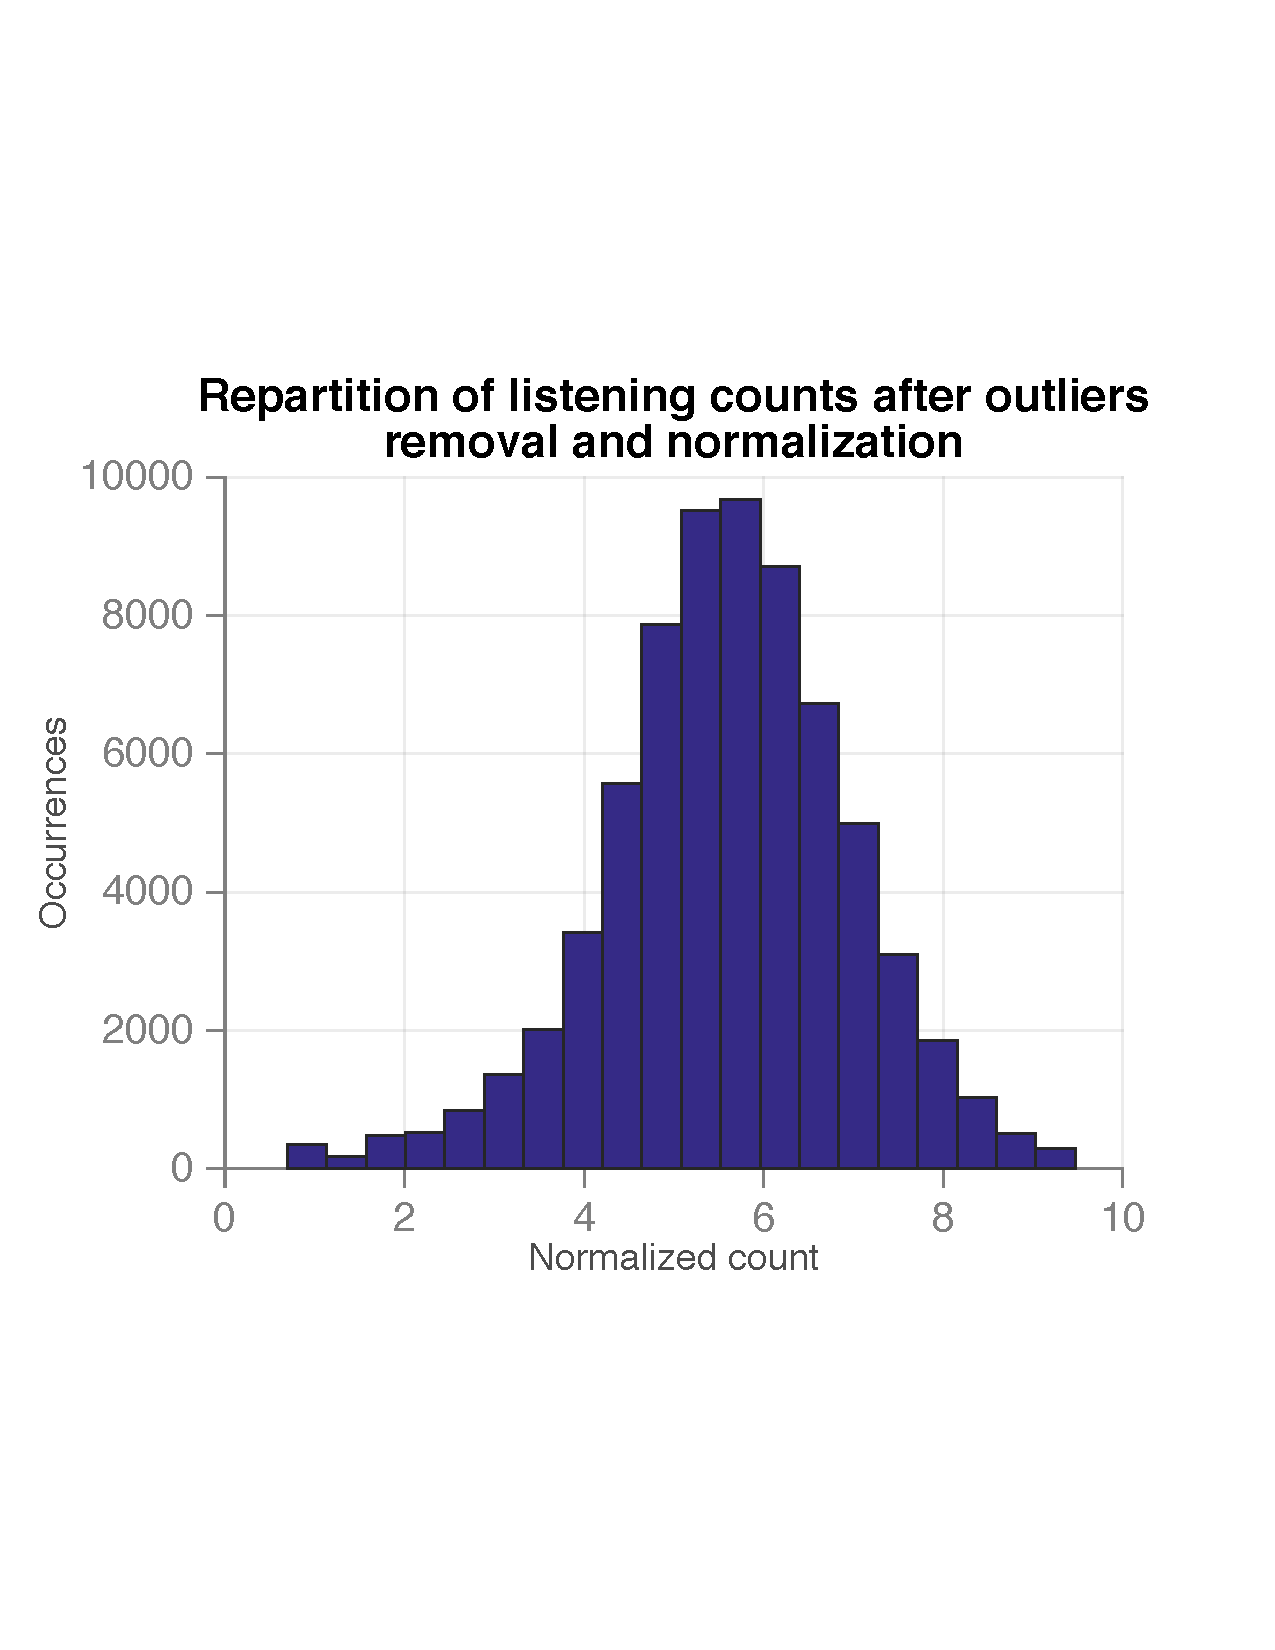
\includegraphics[width=2.5in]{figures/recommendation/normalized-counts.pdf}
    }
    \caption{Normalization makes listening counts distribution more Gaussian}
    \label{fig:recommendation-normalization}
  \end{figure}

  Finally, in order to test our models for both weak and strong predictions, we separated the training set in two ways:
  \begin{itemize}
    \item Entirely remove a proportion of users to use them as a strong prediction test set
    \item Withhold a proportion of the remaining (user, artist, listening count) triplets to use them as a weak prediction test set
  \end{itemize}

  \subsection{Feature transformations}

  \subsection{Final model and predictions}



\section{Image classification}

  \subsection{Dataset description}
  \textbf{Objective}: The people detection dataset consists of a set of images associated with a label that indicates whether there is a person or not in the image. Our goal is to predict whether people are present in unseen images.

  \textbf{Data characteristics}: The training set is composed of $8545$ examples. For each of these images, we are provided with the Histogram of Oriented Gradient (HOG) features generated with Piotr's toolbox. In order to work with the HOG features we convert them into a vector. Hence for each image we get a vector of dimensionality equal to $9360$.

  The training dataset includes $9360$ positive images (images with a person on it) encoded with the label $+1$ and $9360$ negative images encoded with the label $-1$. The dataset is heavily imbalanced between the two classes.

  \subsection{Performance Evaluation}
  As our dataset is imbalanced as mentioned above, we are relying on both true-positive (TP) and false-positive (FP) values as indicators of our performance. We are using a measure called Receiver Operating Characteristics and ROC Curves to compare and evaluate our classifiers' performances. The ideal working point is the top-left corner of the plot where no misclassification is made, thus a classifier that is closer to that point is doing better.

    \subsection{Dataset pre-processing}
  From our data exploration analysis, we did not spot any obvious outliers. All the examples of the training dataset lie between 2 and 3 standard deviations from the median.

  We tried several feature transformations: $log$, $exp$, $sqrt$ and the square of the input features but none of those seemed to help so we decided to keep working with the original features.
  TODO: check exp might be useful when using PCA (at least with 50 features)

  We normalized our data before applying any model to it.

  \subsection{Principal Component Analysis}
  Our features matrix is of dimensionality $9360$ for $8545$ examples which gives us a fat matrice. As several Machine Learning algorithms' time complexity grows fast with dimensionality we applied a Principal Component Analysis on our data in order to work with a low rank approximation of our features. To do so, we used Piotr's $pca()$ implementation which proved to be faster on big datasets. We decided to keep the $NTOREPLACE$ first principal components to project our data on. TODO: Plot explained variance + find value by kCV ?.
  Using a reduced number of features also prevents our classifier to overfit.

   \subsection{Model selection}
   We applied several different classifiers on our data that we have compared to find the best model to make our predictions from. We started from a simple model which is Logistic Regression and then applied Gaussian Processes Classification using Rasmussen's GPML library, Support Vector Machines using LIBSVM toolbox, Neural Networks thanks to the Deep Learning toolbox, and Random Forests. [LIENS EN REF VERS LES TOOLBOXS]

   \textbf{General Approach}:
     	\begin{itemize}
		\item Applying a default implementation of the model to normalized input data or reduced input data after applying PCA depending on computation complexity and performance
    		\item Tuning model parameters: for parameters that seemed relevant on our classifier improvement, we define a range of values to find the best combination thanks to cross validation. As training the different models is rather slow, we used 3-fold cross validation. Other parameters were set manually. We plot learning curves and select the parameter or the best parameter as the one that maximize the average TPR on the test set.
		\item Validating the trained model using 3-fold cross-validation: we computed an average ROC curve over train and test data with a shadowed uncertainty set as 2 standard deviations in order to cover a 95\% confidence interval. This is performed through our kCVfastROC Matlab function.
		\item Finally, we compare the model with other classifiers plotting a ROC Curve for each of them
	\end{itemize}

   \textbf{Logistic Regression}: It turns out that it is just a single-layer Neural Network which is how we implemented it using the Deep Learning toolbox. We added a regularization term, we will see in the Neural Network section how to do so.

   \textbf{Gaussian Processes}: Having a large number of data examples in our training set, we used large scale GP classification that relies on low-rank and diagonal approximation to the exact covariance using induction points. Solving a classification problem, we opted for a logistic function as a likelihood function. We did not had any intuition about the prior distribution so we used a 0-constant mean for our model. We selected a squared exponential covariance with isometric distance measure $covSEiso$ because it uses only two hyper-parameters in comparison to the squared exponential covariance with Automatic Relevant Distance that needs $D+1$ hyper parameters and thus might lead to overfitting. Finally we used Laplace approximation to infer on our data because it provided us with a fairly reasonable computation time compared to the Expectation-Propagation algorithm even if this previous one provided slightly better results.
   ~ may not explain how each hyperparam works... [WHY ALL PARAMETERS?]

    \textbf{Support Vectors Machines}: We first tried to use different kernels: linear, polynomial and Radial Basis function. As the polynomial and RBF kernels are more complex models their computational complexity is much higher than the linear one. Hence we applied SVM with those kernels on our low-rank approximation data. We chose the RBF kernel because it was giving the best performance results [FIGURE?] and then we select the best smoothness parameter $\gamma$ over a range of possible values through cross validation.

    \textbf{Random Forests}: TODO
    number of trees
    fraction of variables in random bagging
    minLeaf
    Learning parameters with kCV

   \textbf{Neural Networks}: We applied a 2-layered Neural Network on our full-dimension data. We were able to tune the number of activation functions on each layer as well as its type: A sigmoid activation function gives better results than the $tanh$[WHY?]. To prevent the Neural Network to overfit, we resort to balance between 2 regularization methods:
   \begin{itemize}
    	\item Applying a weight decay on the second layer which is a Tikhonov regularization
	\item Defining a dropout fraction which removes randomly some activation functions during the training [REF PAPER + check formulation of what it does]
    \end{itemize}
	The best combination of weight decay and dropout fraction parameters has been selected from ranges of parameters using cross-validation as described in the general approach section [REF].

   \textbf{Models comparison}: TODO
   - Plot ROC Curves with the different models, compare, check variance + Random guessing as a base model for comparison
   + Discuss which was difficult or not

  \subsection{Final model and predictions}



\section{Summary}
  Sparse matrix representation made manipulation less straightforward and required us to learn a few new techniques.

  \subsubsection*{Acknowledgments}

  \subsubsection*{References}



\end{document}
